\documentclass[11pt, a4paper]{report}
\usepackage{graphicx}
\usepackage[table,xcdraw]{xcolor}
\usepackage{geometry}
\usepackage[backend=biber]{biblatex}
\usepackage{float}
\usepackage{authblk}
\usepackage{anyfontsize}
\usepackage[document]{ragged2e}
\usepackage{titlesec}
\usepackage[parfill]{parskip}
\usepackage{color}   %May be necessary if you want to color links
\usepackage{hyperref}
\usepackage{caption}
\usepackage{tabularx}
\usepackage{blindtext}
\hypersetup{
    colorlinks=true, %set true if you want colored links
    linktoc=all,     %set to all if you want both sections and subsections linked
    linkcolor=black,  %choose some color if you want links to stand out
}
\titleformat{\chapter}[hang] 
{\normalfont\huge\bfseries}{\chaptertitlename\ \thechapter:}{1em}{} 
\geometry{left=2.5cm,right=2.5cm,top=2.5cm,bottom=2.5cm}
\graphicspath{ {./images/} }

\addbibresource{bibfolder/ref.bib}


% Handy link: https://artofproblemsolving.com/wiki/index.php/LaTeX:Layout

% CHECK https://www.youtube.com/watch?v=ZYvS52511oQ FOR INFO ON SETTINGS FOR biblatex


\begin{document}
\pagestyle{empty}
\centering
\fontsize{2cm}{2cm}\selectfont{Plan of Approach} \\
\vspace{2mm}
\fontsize{1cm}{1cm}\selectfont Audio digital signal processor \\
\vspace{2mm}
\large BeCreative Minor\\
\normalsize
\vspace{4cm}
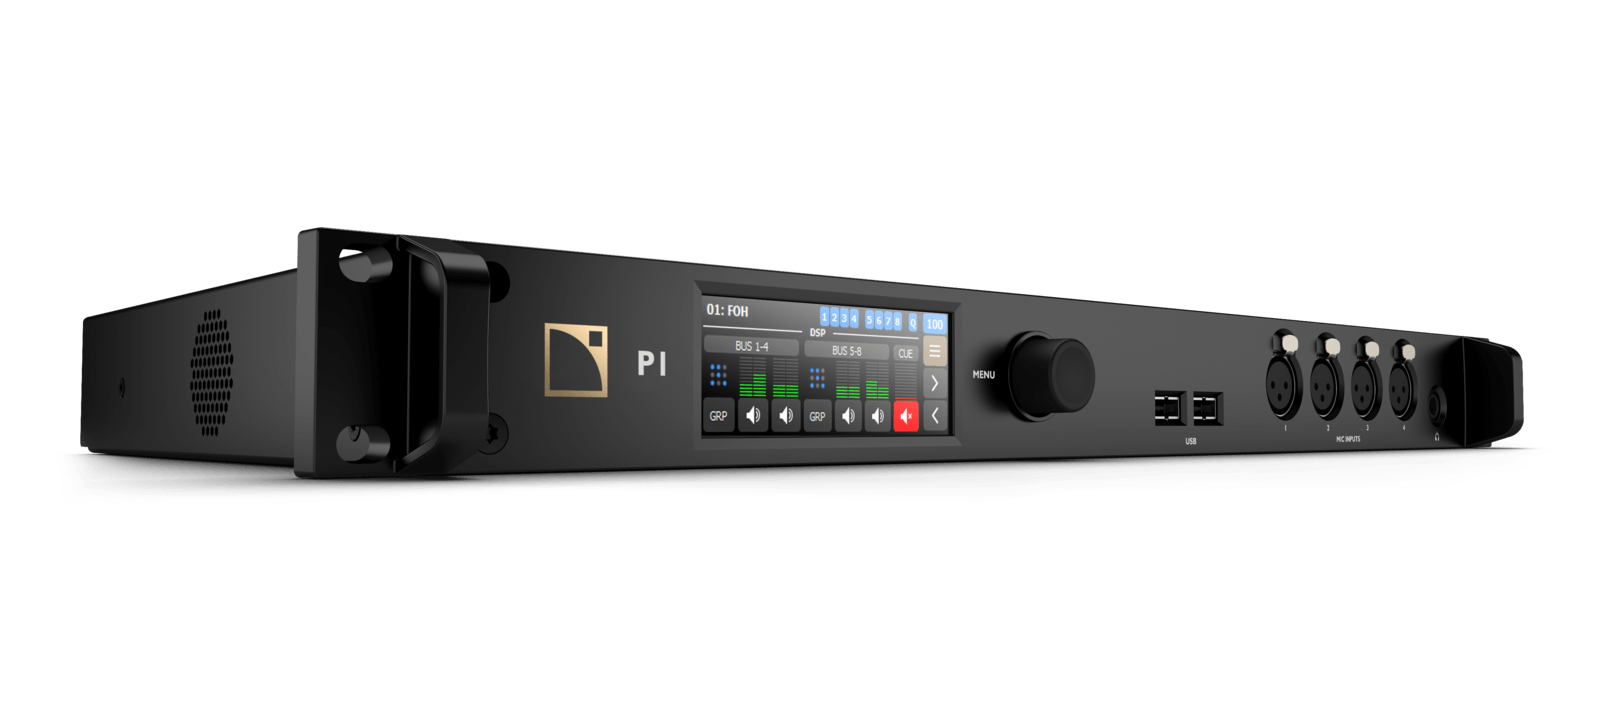
\includegraphics[width=\linewidth]{3DR_P1_Perspective.png}\\
\vfill
\normalsize Busse Lommers \\
Robin van den Dungen \\
Mahmud Gürler \\
Silas Kamphuis \\
Hein Verhallen \\
Youri Tils \\
Ahmed Abdelrahim \\
Fontys Hogescholen, De Rondom 1, 5612 AP Eindhoven \\
\today

\begin{justify}


\newpage
\tableofcontents
\thispagestyle{empty}

\listoffigures
\thispagestyle{empty}


\listoftables
\thispagestyle{empty}

\newpage
\pagestyle{plain}
\setcounter{page}{1}

\chapter*{Abbreviation List}

\begin{table}[!h]
	\centering
\begin{tabular}{|c|c|}
	\hline
\textbf{Abbreviation} & \textbf{Explanation}        \\ \hline
DSP                   & Digital Signal Processor    \\ \hline
ADC                   & Analog-to-Digital Converter \\ \hline
DAC                   & Digital-to-Analog Converter \\ \hline
\end{tabular}
\caption{List of commonly used Abbreviations}
\label{Abbreviation list}
\end{table}

\chapter{Background}
	%BACKGROUND
When listening to music it is of great importance that the speakers are tuned to the environment and the position of the listener. This is necessary to achieve the best experience. If the speakers are not correctly tuned to the surrounding environment, a digital signal processor (DSP) is used to correct this. A DSP is a specialized processor which is used for digital signal processing. 

In the audio world a DSP is used to optimize a sound system. For example some speakers have some imperfections and a DSP can be used to correct for these imperfections. It is also often used to add more dynamics to sound.


\chapter{Project result}
	The goal of this project is to research how to make an audio-DSP. This raises the main research question: \textbf{“How to design an audio-DSP?”}. In the process of researching this an actual audio-DSP will be developed. From the main research question the following sub-research questions are derived:
\begin{itemize} %THIS IS TO MAKE LISTS
	\setlength\itemsep{-0.3em} %MAKES THE GAP SMALLER BETWEEN 2 ITEMS
	\item What is the best method for creating digital filters?
	\item What is the best method for creating digital effects?
	\item What is the most suitable anti-aliasing filter?
	\item What is the optimal needed roll-off for the anti-aliasing filter for a given bandwidth such that the noise can be negligible?
	\item What is the minimum sample frequency needed to capture the desired frequency spectrum?
	\item What is the minimum frequency range to be sampled to achieve sufficient detailed audio?
	\item What is the lowest allowable noise for decent audio?
	\item What analog to digital converter (ADC) resolution is needed such that the quantization error and noise level are on par?
	\item What ADC and digital to analog converter (DAC) architecture is most suitable for this application?
	\item What kind of processor is most suitable for this application?
	\item What is the permittable jitter for accurate audio?
	\item What is the maximum allowable ripple on the reference voltage for the ADC and DAC?
	\item How much RAM does the system need?
	\item How much flash does the system need?
	\item What power supply topology is best suited for each part of the system? \\
\end{itemize}

\noindent
The project is conducted during the minor BeCreative at Fontys. This minor takes 20 weeks and allows the students to have a budget of €300,-. Thus after 20 weeks starting from 6-2-2023 an audio-DSP will be delivered within a budget of €300,-.
\par
\noindent
The audio system has some requirements to specify the final result. These requirements are derived with the “MoSCoW” method. It must be noted that the following requirements will be confirmed by the research that will be conducted.

	\newpage
	\section{Requirements}
	\begin{longtable}{|c|p{10cm}|c|c|}
		\hline
		\textbf{ID} & \textbf{Requirement} & \textbf{Priority} & \textbf{Status}\\ \hline 
		\textbf{U1} & \textbf{Inputs:} \newline
		•Two RCA audio inputs which work on a line level of 4dBu(±1,74V)\newline
		•Two 6,35mm TRS plug audio inputs which work on a line level of 4dBu(±1,74V)\newline
		•Two XLR audio inputs which work on a line level of 22dBu(±9,75)\newline
		•USB type B audio input & Must & Proposed\\ \hline

		\textbf{U2} & \textbf{Outputs:} \newline
		•Two RCA audio outputs which work on a line level of 4dBu(±1,74V)\newline
		•Two 6,35mm TRS plug audio outputs which work on a line level of 4dBu(±1,74V)\newline
		•Four XLR signal outputs which work on a line level of 22dBu(±9,75)
		 & Must & Proposed\\ \hline

		\textbf{U3} &The system should have a bandwidth (±3 dB) of at least 20 Hz up and till 20 kHz without any filters applied. 	& Must   & Proposed\\ \hline
		\textbf{U4} &The system has an Audio sample rate of at least 44.1 kHz 														& Must   & Proposed\\ \hline
		\textbf{U5} &The ADC and DAC resolution is at least 16-bit 																	& Must   & Proposed\\ \hline
		\textbf{U6} &The system has a propagation delay of less than 100ms without any filters applied 								& Must   & Proposed\\ \hline
		\textbf{U7} &User can select what input will be used via a user interface													& Must   & Proposed\\ \hline
		\textbf{U8} &User can select up to 4 effects to active on one channel at the same time 										& Must   & Proposed\\ \hline
		\textbf{U9} &User can configure each effect 																				& Must   & Proposed\\ \hline
		\textbf{U10} &The system must work stand alone and be configurable via a basic graphical user interface 					& Must   & Proposed\\ \hline
		\textbf{U11} &Effects are configurable per output channel, at least four different sound effects should be able to be applied to each signal output signal at the same time: \newline
		\begin{itemize}
			\setlength\itemsep{-0.4em}
			\item Distortion
			\item Reverb
			\item Gain
			\item Equalizer
			\item Delay
		\end{itemize}																												& Must 	 & Proposed\\ \hline
		\textbf{U12}  &The system should have a bandwidth (±1 dB) of at least 20 Hz up and till 20 kHz without any filters applied 	& Should & Proposed\\ \hline
		\textbf{U13}  &Audio sample rate of at least 96 kHz 																		& Should & Proposed\\ \hline
		\textbf{U14} & The ADC and DAC resolution is at least 24-bit. 																& Should & Proposed\\ \hline
		\textbf{U15} & Six XLR signal outputs work on a line level of 22 dBu (±9,75 V) 												& Should & Proposed\\ \hline
		\textbf{U16} & User can select up to 10 effects to be active in one channel at the same time. 								& Should & Proposed\\ \hline
		\textbf{U17} & Low enough jitter to not influence the audio quality too much 												& Should & Proposed\\ \hline
		\textbf{U18} & Local power supplies for different parts of the system 														& Should & Proposed\\ \hline
		\textbf{U19} & Low enough jitter to not influence the audio quality too much 												& Should & Proposed\\ \hline
		\textbf{U20} & Effects:\newline
		\begin{itemize}
			\setlength\itemsep{-0.3em}
			\item Phaser
			\item Tremelo
			\item Flanger
			\item Fuzz
			\item Overdrive
			\item Chorus
			\item Compressor
			\item Wah
			\item Looper
			\item Wow and flutter
			\item Modulator
			\item Echo
			\item Fade in
		\end{itemize}																												& Should & Proposed\\ \hline
		\textbf{U21} & Audio sample rate of at least 192 kHz 																		& Could  & Proposed\\ \hline
		\textbf{U22} & Touch screen user interface 																					& Could  & Proposed\\ \hline
		\textbf{U23} & Self-made mains power supply  																				& Won't  & Proposed\\ \hline
	\end{longtable}
	
\chapter{Project activities}
	In order to realise this project, the activities need to be devised. describing the end-product in precise terms will make it easier to devise those tasks. These activities are: 

\begin{itemize}
	\setlength\itemsep{-0.2em}
	\item Planning
	\item Research
	\item Designing
	\item Testing
	\item Writing documentation
	\item Budget tracking
\end{itemize}


	\section{Planning}
	
The planning is one of the most important stages within the project activities, this gives you the broad overview over the whole project and what it is going to look like. In order to determine the activities, progress, costs, duration and delay of a project, a planning is of the essence. 
The planning will be divided into two separate parts:

\begin{itemize}
	\setlength\itemsep{-0.2em}
	\item Global planning
	\item Personal (weekly or daily) planning
\end{itemize}
\noindent
The global planning will be made in Gantt-chart style. The personal planning is freer of choice depended on the team member itself.
	
	
	\section{Research}
	
In chapter 2 Project result the research questions are described. Those questions need to be answered before specifying the things that are needed to start working on this project. This phase is especially important because of its responsibility that it carries in future development of the project. The better the research is done, the less wrongly things will be executed in the future stage of the project, which will save time. 
The research questions will be separated in two categories: 

\begin{itemize}
	\setlength\itemsep{-0.2em}
	\item The research questions that will be split into the team members that have the interest in the specific subject based on their PDP.
	\item The research questions that needed to be discussed in a group matter, so everyone is on par with the research and knowledge.
\end{itemize}


	\section{Designing}
	
During this stage most of the research will have been completed and the tasks will be divided into the team members. Depended on the PDP and the preferred modules the team members will work either together or alone on a module. While designing the other team members will be updated in the weekly meetings. 
	
	\section{Testing}
	
After the design phase the modules will be put together and will be tested based on the test report.
	% \cite{fontys}
	
	\section{Writing Documentation}
	
If all the necessary requirements (user and functional) are fulfilled and testing is done, the evidence will be put in the final report.
	
	\section{Budget tracking}
	
Fontys has provided us with a budget of €300, - for the completion of this project. The most expensive parts expected will be the processor, the ADC’s and the DAC’s.


	

\chapter{Project boundaries}
	The needed mains power supply will not be made during this project and will be bought externally.

\noindent For the power supply a transformer is used to make a safe voltage.

	
\chapter{Milestones}
	%Milestones
<<<<<<< Updated upstream
The following milestones will be achieved as a result of the project activities as in Chapter 3.
\begin{itemize}
    \setlength\itemsep{-0.2em}
    \item Reports:
    \begin{itemize}
        \setlength\itemsep{-0.2em}
        \item Research document
        \item SRD
        \item SDD
        \item MDD
        \item Final report
    \end{itemize}
    \item Designs:
    \begin{itemize}
        \setlength\itemsep{-0.2em}
        \item Firmware design:
        \begin{itemize}
            \setlength\itemsep{-0.2em}
            \item Input MUX design
            \item Sampler design
            \item USB decoder design
            \item Output MUX design
            \item signal processor design
            \begin{itemize}
                \setlength\itemsep{-0.2em}
                \item Effect manager design
                \item Effects design/model
                \item Filters design/model
            \end{itemize}
            \item controller design
        \end{itemize}
        \item Hardware design:
        \begin{itemize}
            \setlength\itemsep{-0.2em}
            \item Input selector design
            \item Anti-aliasing filters design
            \item Output filter design
            \item Buffer design
            \item XLR balanced-to-unbalanced converter design
            \item XLR unbalanced-to-balanced converter design
            \item processor core design
            \item Local power supplies design
            \item Housing design
        \end{itemize}
        \item User interface design
    \end{itemize}
    \item Realistation:
    \begin{itemize}
        \setlength\itemsep{-0.2em}
        \item Firmware:
        \begin{itemize}
            \setlength\itemsep{-0.2em}
            \item Program ADC and DAC interface
            \item Program sampler
            \item Program USB decoder
            \item Program MUX
            \item Program signal processor
            \begin{itemize}
                \setlength\itemsep{-0.2em}
                \item Program effect manager
                \item Program filters
                \item Program effects
            \end{itemize}
            \item Program controller
        \end{itemize}
        \item Hardware:
        \begin{itemize}
            \setlength\itemsep{-0.2em}
            \item Housing
            \item PCB
        \end{itemize}
        \item User interface
    \end{itemize}
\end{itemize}
=======
The following milestones will be achieved as a result of the project activities described in chapter 3.\\

\begin{itemize}
	\setlength\itemsep{-0.3em}
	\item Reports
	\begin{itemize}
		\setlength\itemsep{-0.3em}
		\item Research document
		\item SRD
		\item SDD
		\item MDD
		\item Creating final report
	\end{itemize}
	\item Designs
	\begin{itemize}
		\setlength\itemsep{-0.3em}
		\item Firmware design:
		\begin{itemize}
			\setlength\itemsep{-0.3em}
			\item Input MUX design
			\item Sampler design
			\item USB decoder design
			\item Output MUX deisgn
			\item Signal processor design:
			\begin{itemize}
				\setlength\itemsep{-0.3em}
				\item Effect manager design
				\item Effects design/model
				\item Filter design/model
			\end{itemize}
			\item Controller design
		\end{itemize}
		\item Hardware design:
		\begin{itemize}
			\setlength\itemsep{-0.3em}
			\item Input selector design
			\item Anti-aliasing filters design
			\item Output filter design
			\item Buffer design
			\item XLR balanced-to-unbalanced converter design
			\item XLR unbalanced-to-balanced converter design
			\item Processor core design
			\item Local power supplies design
			\item Housing design
		\end{itemize}
		\item User interface design
	\end{itemize}
	\item Realisation
	\begin{itemize}
		\setlength\itemsep{-0.3em}
		\item Firmware:
		\begin{itemize}
			\setlength\itemsep{-0.3em}
			\item Program ADC and DAC interface
			\item Program sampler
			\item Program USB decoder
			\item Program MUX
			\item Program signal processor:
			\begin{itemize}
				\setlength\itemsep{-0.3em}
				\item Program effect manager
				\item Program filters
				\item Program effects
			\end{itemize}
			\item Program controller 
		\end{itemize}
		\item Create hardware:
		\begin{itemize}
			\setlength\itemsep{-0.3em}
			\item Housing
			\item PCB
		\end{itemize}
		\item User interface 
	\end{itemize}
\end{itemize} 


>>>>>>> Stashed changes


\chapter{Quality assurance}
	%Quality Assurance

\chapter{Project organisation}
	\begin{itemize}
    \setlength\itemsep{-0.3em}
    \item Weekly meetings
    \item Roles within the project:
    \begin{itemize}
        \setlength\itemsep{-0.3em}
        \item Communicator
        \item Minute-taker
        \item Chairman/project-leader
        \item Accountant\\
    \end{itemize}
\end{itemize}

\begin{table}[!h]
    \begin{tabular}{|l|l|l|}
        \hline
        \textbf{Role} & \textbf{Assigned person} & \textbf{Back-up person}\\ \hline
        Communicator & Robin van den Dungen & Silas Kamphuis\\ \hline
        Minute-taker & Ahmed Abdelrahim & Mahmud Gürler\\ \hline
        Chairman/project-leader & Youri Tils & Robin van den Dungen\\ \hline
        Accountant & Hein Verhallen & Silas Kamphuis\\ \hline
        Editor & Busse Lommers & Hein Verhallen\\ \hline
        Version-controller & Hein Verhallen & Youri Tils\\ \hline
    \end{tabular}
    \caption{Role division}
\end{table}

\chapter{Planning}
	%orange : FF9930
\arrayrulecolor{black}
    \begin{table}[!h]
        \textcolor{white}{
            \begin{tabular}{l|l|l|l|l|l|l|l|l|l|l|l|l|l|l|l|l|l|l|l|}
            \cline{2-20}
             & \multicolumn{19}{c|}{\cellcolor{cyan}Project Week Number}                                                             \\ \hline
             \rowcolor{cyan}
             \multicolumn{1}{|l|}{\cellcolor{cyan}Activities}               &1 &2 &3 &4 &5 &6 &7 &8 &9 &10&11&12&13&14&15&16&17&18&19\\ \hline
             \rowcolor{orange}
             \multicolumn{1}{|l|}{\cellcolor{cyan}Plan of Approach}         &\cellcolor{orange}&\cellcolor{orange}&&&&&&&&&&&&&&&&&  \\ \hline
             \multicolumn{1}{|l|}{\cellcolor{cyan}Researching}              &&\cellcolor{orange}&\cellcolor{orange}&\cellcolor{orange}&&&&&&&&&&&&&&&  \\ \hline
             \multicolumn{1}{|l|}{\cellcolor{cyan}Design firmware}          &&&&\cellcolor{orange}&\cellcolor{orange}&\cellcolor{orange}&\cellcolor{orange}&\cellcolor{orange}&\cellcolor{orange}&\cellcolor{orange}&\cellcolor{orange}&\cellcolor{orange}&&&&&&&  \\ \hline
             \multicolumn{1}{|l|}{\cellcolor{cyan}Design hardware}          &&&&\cellcolor{orange}&\cellcolor{orange}&\cellcolor{orange}&\cellcolor{orange}&\cellcolor{orange}&\cellcolor{orange}&\cellcolor{orange}&\cellcolor{orange}&\cellcolor{orange}&&&&&&&  \\ \hline
             \multicolumn{1}{|l|}{\cellcolor{cyan}Program user interface}   &&&&\cellcolor{orange}&\cellcolor{orange}&\cellcolor{orange}&\cellcolor{orange}&\cellcolor{orange}&\cellcolor{orange}&\cellcolor{orange}&\cellcolor{orange}&\cellcolor{orange}&&&&&&&  \\ \hline
             \multicolumn{1}{|l|}{\cellcolor{cyan}Design user interface}    &&&&&&&&&&&&\cellcolor{orange}&\cellcolor{orange}&\cellcolor{orange}&\cellcolor{orange}&\cellcolor{orange}&\cellcolor{orange}&\cellcolor{orange}&  \\ \hline
             \multicolumn{1}{|l|}{\cellcolor{cyan}Program firmware}         &&&&&&&&&&&&\cellcolor{orange}&\cellcolor{orange}&\cellcolor{orange}&\cellcolor{orange}&\cellcolor{orange}&\cellcolor{orange}&\cellcolor{orange}&  \\ \hline
             \multicolumn{1}{|l|}{\cellcolor{cyan}Create hardware}          &&&&&&&&&&&&\cellcolor{orange}&\cellcolor{orange}&\cellcolor{orange}&\cellcolor{orange}&\cellcolor{orange}&\cellcolor{orange}&\cellcolor{orange}&  \\ \hline
             \multicolumn{1}{|l|}{\cellcolor{cyan}Testing}                  &&&&&&&&&&&&&&&&&&\cellcolor{orange}&\cellcolor{orange}  \\ \hline
            \end{tabular}
        }
        \caption{Planning}
        \end{table}

\chapter{Cost-benefit overview}
	From Fontys we get a budget of €300, - for this project. The most expensive parts will be the FPGA, the ADC’s and the DAC’s.  

\chapter{Risk Analysis}
	%FILE FOR RISK ANALYSIS
There are many risks and reasons why a project might fail or go bad, A change in organizational priorities is the most common reason. A change in project objectives is also common as poor communication and unclear risk definition.
	\begin{itemize}
		\setlength\itemsep{-0.3em}
		\item Unclear or shifting goals.
		\item lack of planning.
		\item lack of follow up.
		\item timing issues 
		\item Lack of risk management.
		\item Unsuitable tools.
		\item Too many unsuitable tools
	\end{itemize}

\noindent
For these reasons and many more, we’ve created an overall table with ratings which rate the opportunity/effect and risk.
	
% Please add the following required packages to your document preamble:
% \usepackage{graphicx}
% \usepackage[table,xcdraw]{xcolor}
% If you use beamer only pass "xcolor=table" option, i.e. \documentclass[xcolor=table]{beamer}
% \begin{table}[!h]
% \centering
% \resizebox{\textwidth}{!}{%
% \begin{tabular}{|l|
% >{\columncolor[HTML]{9AFF99}}l |l|l|l|
% >{\columncolor[HTML]{9AFF99}}l |
% >{\columncolor[HTML]{9AFF99}}l |l|}
% \hline
% \cellcolor[HTML]{CBCEFB}Risk                                                                       & \cellcolor[HTML]{CBCEFB}Opportunity & \cellcolor[HTML]{CBCEFB}Effects & \cellcolor[HTML]{CBCEFB}Risk & \cellcolor[HTML]{CBCEFB}\begin{tabular}[c]{@{}l@{}}Measure to prevent /\\ Remedy it\end{tabular}                                                                 & \cellcolor[HTML]{CBCEFB}Change after & \cellcolor[HTML]{CBCEFB}Consequences afterwards & \cellcolor[HTML]{CBCEFB}Ultimate risk \\ \hline
% \begin{tabular}[c]{@{}l@{}}A group member\\ lacks in work / failed\\ deadlines.\end{tabular}       & \cellcolor[HTML]{FFFC9E}4           & \cellcolor[HTML]{9AFF99}2       & \cellcolor[HTML]{FFCCC9}8    & \begin{tabular}[c]{@{}l@{}}Code of conduct created and\\ singed by everyone\end{tabular}                                                                         & 3                                    & 3                                               & \cellcolor[HTML]{FFFC9E}4             \\ \hline
% \begin{tabular}[c]{@{}l@{}}Clear file locations\\ and easy to map.\end{tabular}                    & 3                                   & \cellcolor[HTML]{9AFF99}3       & \cellcolor[HTML]{FFFC9E}6    & \begin{tabular}[c]{@{}l@{}}Weekly document tracking\\ and documentation is taken.\end{tabular}                                                                   & 2                                    & 3                                               & \cellcolor[HTML]{9AFF99}3             \\ \hline
% \begin{tabular}[c]{@{}l@{}}Behind schedule for\\ lack of knowledge or\\ confusion.\end{tabular}    & 4                                   & \cellcolor[HTML]{9AFF99}3       & \cellcolor[HTML]{FFCCC9}7    & \begin{tabular}[c]{@{}l@{}}Ask for help in time from\\ fellow group members or\\ teachers.\end{tabular}                                                          & 1                                    & 2                                               & \cellcolor[HTML]{9AFF99}2             \\ \hline
% Running low on budget.                                                                             & 1                                   & \cellcolor[HTML]{FFFC9E}6       & \cellcolor[HTML]{9AFF99}5    & Budget is documented.                                                                                                                                            & 1                                    & 3                                               & \cellcolor[HTML]{9AFF99}1             \\ \hline
% \begin{tabular}[c]{@{}l@{}}There is insufficient\\ communication in the\\ group.\end{tabular}      & 2                                   & \cellcolor[HTML]{9AFF99}3       & \cellcolor[HTML]{FFFC9E}6    & \begin{tabular}[c]{@{}l@{}}Meetings will be scheduled 2-3\\ times a week, minutes and\\ notes are taken and uploaded\\ up to date.\end{tabular}                  & 1                                    & 3                                               & \cellcolor[HTML]{9AFF99}3             \\ \hline
% \begin{tabular}[c]{@{}l@{}}Clear results are\\ missing.\end{tabular}                               & \cellcolor[HTML]{FFFC9E}4           & \cellcolor[HTML]{FFFC9E}6       & \cellcolor[HTML]{FFCCC9}9    & \begin{tabular}[c]{@{}l@{}}The strip planning clearly\\ states which part you need to\\ complete to be on schedule\\ with each part of the project.\end{tabular} & 2                                    & 3                                               & \cellcolor[HTML]{FFFC9E}6             \\ \hline
% \begin{tabular}[c]{@{}l@{}}Shortage in\\ components\end{tabular}                                   & 2                                   & \cellcolor[HTML]{FFCCC9}9       & \cellcolor[HTML]{9AFF99}3    & \begin{tabular}[c]{@{}l@{}}A delay in ordering or\\ receiving parts\end{tabular}                                                                                 & \cellcolor[HTML]{FFFC9E}6            & \cellcolor[HTML]{FFFC9E}6                       & \cellcolor[HTML]{FFCCC9}9             \\ \hline
% \begin{tabular}[c]{@{}l@{}}The planning of\\ Fontys teaching\\ material is incorrect.\end{tabular} & \cellcolor[HTML]{FFFC9E}4           & \cellcolor[HTML]{FFFC9E}5       & \cellcolor[HTML]{FFCCC9}9    & Read documents carefully                                                                                                                                         & \cellcolor[HTML]{FFFC9E}4            & \cellcolor[HTML]{FFCCC9}7                       & \cellcolor[HTML]{FFCCC9}7             \\ \hline
% \end{tabular}%
% }
% \caption{Risk analysis}
% \label{Risk analysis}
% \end{table}

\newpage
\begin{table}[!h]
	\centering
	\begin{tabular}{|>{\columncolor{gray}}c|c|c|c|c|c|}
		\cline{2-6}
		\rowcolor{gray}
		\multicolumn{1}{l|}{\cellcolor{white}}&Very low&Low		&Medium					&High					&Very high 				\\ \hline
		Very likely	&\cellcolor{yellow}5&\cellcolor{orange}10	&\cellcolor{red}15		&\cellcolor{red}20		&\cellcolor{red}25 		\\ \hline
		likely		&\cellcolor{green}4	&\cellcolor{yellow}8	&\cellcolor{orange}12	&\cellcolor{red}16		&\cellcolor{red}20 		\\ \hline
		possible	&\cellcolor{green}3	&\cellcolor{yellow}6	&\cellcolor{yellow}9	&\cellcolor{orange}12	&\cellcolor{red}15 		\\ \hline
		Unlikely	&\cellcolor{green}2	&\cellcolor{green}4		&\cellcolor{yellow}6	&\cellcolor{yellow}8	&\cellcolor{orange}10	\\ \hline
		Rare		&\cellcolor{green}1	&\cellcolor{green}2		&\cellcolor{green}3		&\cellcolor{green}4		&\cellcolor{yellow}5	\\ \hline
	\end{tabular}
	\caption{risk analysis index}
\end{table}

\begin{table}[!h]
	\begin{tabularx}{\textwidth}{|c|X|X|c|c|c|} \hline
		\# 	& Risk 													& Action 																										& Probability 	& Impact 	& Score \\ \hline
		1 	& A group member lacks in word/failed deadlines		& Code of Conduct created and signed by everyone																& 4				& 2			& 8		\\ \hline
		2 	& Clear file locations and easy to map					& Weekly document tracking and documentation is taken															& 3				& 3			& 9		\\ \hline
		3 	& Behind schedule for lack of knowledge or confusion	& Ask for help in time from fellow group members or teachers													& 4				& 3			& 12	\\ \hline
		4 	& Running low on budget									& Budget is documented																							& 1				& 5			& 5		\\ \hline
		5 	& There is insufficient communication in the group		& Meetings scheduled 2-3 times a week, Minutes and notes are taken and uploaded up to date						& 2				& 3			& 6		\\ \hline
		6 	& Clear results are missing								& The stip planning clearly states which part you need to complete to be on schedule with your project component& 4				& 2			& 8		\\ \hline
		7 	& Shortage in components								& A delay in ordering or receiving parts																		& 2				& 5			& 10	\\ \hline
		8 	& The planning of Fontys teaching material is incorrect	& Read documents carefully																						& 4				& 2			& 8		\\ \hline
	\end{tabularx}
	\caption{Risk analysis}
\end{table}

% Bibliography with heading so it pops up in the table of contents (i don't know why but this is how it works)
\printbibliography[
heading=bibintoc,
title={Bibliography}
]
	\end{justify}
\end{document}
